\documentclass[conference]{IEEEtran}
\usepackage{amsmath,amssymb}
\usepackage{booktabs}
\usepackage{graphicx}
\usepackage{tikz}
\usepackage{algorithm}
\usepackage{algpseudocode}
\usetikzlibrary{arrows.meta,positioning,shapes.geometric}

\title{Methodology -- Adaptive Staleness-Aware Gradient Compression for Asynchronous Distributed Training}
\author{%
\begin{tabular*}{\textwidth}{@{\extracolsep{\fill}}cccc@{}}
\parbox[t]{0.22\textwidth}{\centering
\textbf{G. Bhavana}\\[-1pt]
(241IT029)\\[-1pt]
\textit{dept. of Information Technology}\\[-1pt]
\textit{National Institute of Technology}\\[-1pt]
\textit{Karnataka, Surathkal}}
&
\parbox[t]{0.22\textwidth}{\centering
\textbf{Sacheth Koushal}\\[-1pt]
(241IT058)\\[-1pt]
\textit{dept. of Information Technology}\\[-1pt]
\textit{National Institute of Technology}\\[-1pt]
\textit{Karnataka, Surathkal}}
&
\parbox[t]{0.22\textwidth}{\centering
\textbf{Vivaan Sharma}\\[-1pt]
(241IT081)\\[-1pt]
\textit{dept. of Information Technology}\\[-1pt]
\textit{National Institute of Technology}\\[-1pt]
\textit{Karnataka, Surathkal}}
&
\parbox[t]{0.22\textwidth}{\centering
\textbf{Yash Roshan}\\[-1pt]
(241IT083)\\[-1pt]
\textit{dept. of Information Technology}\\[-1pt]
\textit{National Institute of Technology}\\[-1pt]
\textit{Karnataka, Surathkal}}
\end{tabular*}%
}

\begin{document}
\maketitle

\section{Methodology}
\label{sec:methodology}

The proposed framework is an asynchronous parameter-server system that jointly controls gradient compression and gradient staleness. Workers compute local stochastic gradients from independently assigned mini-batches and transmit updates without waiting for other workers. Each update carries the model version from which it was computed. The parameter server uses this version information to measure staleness, attenuate moderately stale updates, and reject excessively stale updates. A runtime controller then adapts the compression level and the allowable staleness from observed training and system conditions. The design follows the project objective of reducing communication cost and straggler impact without materially degrading convergence.

\subsection{Research Workflow}
\label{subsec:workflow}

The research workflow is organized into five stages: workload preparation, asynchronous gradient generation, compression and staleness-aware server processing, runtime adaptation, and controlled evaluation. The same workload and delay schedule are applied to all baselines so that measured differences can be attributed to the training strategy rather than to different data or system conditions.

\begin{figure}[!ht]
\centering
\resizebox{0.98\columnwidth}{!}{%
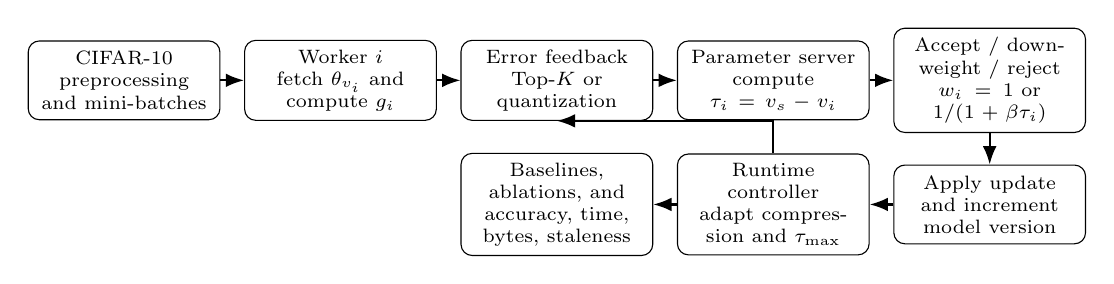
\begin{tikzpicture}[
box/.style={draw,rounded corners,align=center,minimum height=10mm,text width=22mm,font=\scriptsize},
arrow/.style={-Latex,thick}
]
\node[box] (data) {CIFAR-10\\preprocessing and mini-batches};
\node[box,right=3mm of data] (worker) {Worker $i$\\fetch $\theta_{v_i}$ and\\compute $g_i$};
\node[box,right=3mm of worker] (compress) {Error feedback\\Top-$K$ or quantization};
\node[box,right=3mm of compress] (server) {Parameter server\\compute $\tau_i=v_s-v_i$};
\node[box,right=3mm of server] (policy) {Accept / downweight / reject\\$w_i=1$ or $1/(1+\beta\tau_i)$};
\node[box,below=4mm of policy] (update) {Apply update and increment\\model version};
\node[box,left=3mm of update] (control) {Runtime controller\\adapt compression and $\tau_{\max}$};
\node[box,left=3mm of control] (eval) {Baselines, ablations, and\\accuracy, time, bytes, staleness};
\draw[arrow] (data)--(worker);
\draw[arrow] (worker)--(compress);
\draw[arrow] (compress)--(server);
\draw[arrow] (server)--(policy);
\draw[arrow] (policy)--(update);
\draw[arrow] (update)--(control);
\draw[arrow] (control)--(eval);
\draw[arrow] (control.north) |- (compress.south);
\end{tikzpicture}%
}
\caption{Overall methodology for adaptive staleness-aware asynchronous distributed training.}
\label{fig:workflow}
\end{figure}



\subsection{Dataset and Data Preparation}
\label{subsec:dataset}

CIFAR-10 is used as the primary image-classification workload, as specified in the project proposal. The dataset provides a fixed supervised learning task while worker speed and communication conditions can be varied independently. Every method uses the same preprocessing pipeline, model architecture, optimizer, mini-batch size, learning-rate schedule, initialization policy, and training budget. This prevents differences in model quality from being attributed to unrelated changes in the learning setup.

The data are partitioned at mini-batch granularity across workers. Worker $i$ processes mini-batch $B_i$ using the local copy of the model associated with version $v_i$. Its stochastic gradient is
\begin{equation}
 g_i=\nabla_{\theta}\mathcal{L}(\theta_{v_i};B_i).
 \label{eq:gradient}
\end{equation}
The worker does not wait for other workers after computing the gradient. This removes the global barrier present in synchronous SGD and allows faster workers to continue generating updates while slower workers are still processing earlier mini-batches.

Controlled heterogeneity is introduced after the normal data pipeline. Computation delay is inserted before transmission to emulate slower workers, while communication delay or bandwidth constraints are used to emulate network variation. The same delay scenarios are replayed across competing methods.

\subsection{Worker-Side Compression and Error Feedback}
\label{subsec:compression}

Compression is applied to the gradient after error feedback. Let $e_i$ denote the residual stored by worker $i$ from its previous transmission. The vector passed to the compressor is
\begin{equation}
 u_i=g_i+e_i.
 \label{eq:ef}
\end{equation}
If $\mathcal{C}(\cdot)$ is the compressor and $\mathcal{D}(\cdot)$ is the reconstruction operation at the server, the transmitted update represents
\begin{equation}
 \hat g_i=\mathcal{D}\!\left(\mathcal{C}(u_i)\right),
 \qquad
 e_i^{\mathrm{new}}=u_i-\hat g_i.
 \label{eq:residual}
\end{equation}
The residual therefore stores the information discarded in the current transmission and carries it into later updates. Error feedback is used because aggressive sparsification or quantization can otherwise remove small but accumulated gradient components~\cite{aji2017sparse,alistarh2017qsgd,karimireddy2019ef}.

\subsubsection{Top-$K$ Sparsification}
For a gradient vector $u\in\mathbb{R}^{d}$, Top-$K$ keeps the $K$ entries with largest absolute magnitude and suppresses the remaining entries. The selected set is
\begin{equation}
 S_K(u)=\operatorname*{arg\,topK}_{j\in\{1,\ldots,d\}}|u_j|,
\end{equation}
with compressed representation
\begin{equation}
 [\mathcal{C}_K(u)]_j=
 \begin{cases}
 u_j,&j\in S_K(u),\\
 0,&j\notin S_K(u).
 \end{cases}
 \label{eq:topk}
\end{equation}
The control variable is the sparsity fraction $K/d$. Smaller values reduce payload size but increase information discarded per communication step.

\subsubsection{Quantization}
Quantization provides an alternative compression mode in which each value is represented using $b$ bits:
\begin{equation}
 \hat u=Q_b(u).
 \label{eq:quant}
\end{equation}
Reducing $b$ lowers communication volume but increases quantization error. Top-$K$ and quantization are evaluated as separate modes so that the experimental analysis can identify whether improvements arise from sparsity, reduced precision, or the adaptive control policy~\cite{lin2018deep,alistarh2017qsgd}.

\subsection{Server-Side Staleness Control}
\label{subsec:staleness}

The parameter server maintains the authoritative model $\theta_{v_s}$ and a monotonically increasing version number $v_s$. Every update contains the source version $v_i$. The staleness of an arriving update is
\begin{equation}
 \tau_i=v_s-v_i.
 \label{eq:staleness}
\end{equation}
Thus, $\tau_i=0$ denotes an update computed from the current model version, whereas larger values indicate that additional server updates have occurred since the worker started its computation.

Three staleness regions are used. Recent updates are accepted with unit weight. Moderately stale updates are downweighted using
\begin{equation}
 w_i=\frac{1}{1+\beta\tau_i},
 \label{eq:weight}
\end{equation}
where $\beta$ determines the sensitivity to staleness. Updates for which
\begin{equation}
 \tau_i>\tau_{\max}
 \label{eq:reject}
\end{equation}
are rejected. For an accepted update, the server performs
\begin{equation}
 \theta_{v_s+1}=\theta_{v_s}-\eta w_i\hat g_i,
 \label{eq:update}
\end{equation}
and increments the server version. This mechanism preserves asynchronous execution while limiting the influence of gradients computed from substantially older parameter states.

\begin{algorithm}[t]
\caption{Staleness-Aware Server Update}
\label{alg:server}
\begin{algorithmic}[1]
\Require $\theta_{v_s}$, $v_s$, $\beta$, $\tau_{\max}$, learning rate $\eta$
\For{each arriving update $(\mathcal{C}(u_i),v_i)$}
  \State Reconstruct $\hat g_i$ from the received update
  \State $\tau_i\gets v_s-v_i$
  \If{$\tau_i>\tau_{\max}$}
    \State Reject update; increment rejection counter
  \Else
    \If{update is recent}
      \State $w_i\gets1$
    \Else
      \State $w_i\gets1/(1+\beta\tau_i)$
    \EndIf
    \State $\theta_{v_s+1}\gets\theta_{v_s}-\eta w_i\hat g_i$
    \State $v_s\gets v_s+1$
  \EndIf
  \State Update runtime measurements
\EndFor
\end{algorithmic}
\end{algorithm}

\subsection{Joint Runtime Adaptation}
\label{subsec:controller}

The central contribution is a controller that treats compression and staleness tolerance as coupled runtime controls rather than fixed independent hyperparameters. At a fixed control interval, the server records the loss trend, loss variance, average staleness, rejected-update rate, communication time, and update throughput. Let the observed system state be
\begin{equation}
 z_t=\{\Delta L_t,\operatorname{Var}(L)_t,\bar\tau_t,r_t,T_t^{\mathrm{comm}},P_t\}.
 \label{eq:state}
\end{equation}
The next configuration is selected as
\begin{equation}
 c_{t+1}=\pi(z_t)=\left(\text{compression}_{t+1},\tau_{\max,t+1}\right).
 \label{eq:controller}
\end{equation}

When loss remains stable and communication pressure is high, the controller can increase compression strength or relax the staleness threshold. When loss variance or update rejection becomes excessive, it moves toward safer settings. The exact thresholds are experimental parameters and must be fixed before the final benchmark; they are not specified numerically in the proposal. Every controller decision is logged to preserve reproducibility and to permit post-hoc analysis of why a configuration changed.

\subsection{Experimental Settings}
\label{subsec:experiments}

The experimental design isolates the contribution of each mechanism. The same model, optimizer, workload, training budget, initialization, and delay schedule are used for matched comparisons. Independent runs with fixed random seeds are used to quantify stochastic variation.

\begin{table}[t]
\centering
\caption{Comparison and ablation configurations.}
\label{tab:baselines}
\renewcommand{\arraystretch}{1.08}
\begin{tabular}{p{0.23\columnwidth}p{0.67\columnwidth}}
\toprule
\textbf{Configuration} & \textbf{Definition}\\
\midrule
Synchronous SGD & Global synchronization before each update; serves as a straggler-sensitive baseline.\\
Plain asynchronous SGD & Asynchronous parameter server without adaptive staleness control or adaptive compression.\\
Fixed staleness & Fixed $\beta$ and $\tau_{\max}$; compression held constant.\\
Fixed compression & Fixed Top-$K$ level or bit width; staleness policy held constant.\\
Proposed method & Asynchronous updates with staleness control, adaptive compression, adaptive $\tau_{\max}$, and error feedback.\\
Ablation: no EF & Remove the residual term $e_i$ while keeping all other settings unchanged.\\
Ablation: fixed controls & Hold compression or staleness adaptation fixed to isolate each controller contribution.\\
\bottomrule
\end{tabular}
\end{table}

At least two stress dimensions are varied: worker computation delay and communication delay. The purpose is not to imitate a particular production cluster but to create controlled conditions in which stale updates and communication overhead become measurable. Delay levels should be reported explicitly with the final results rather than described only qualitatively.

\subsection{Evaluation and Expected Analysis}
\label{subsec:evaluation}

Model quality is evaluated using final validation accuracy and training loss. Convergence speed is measured by wall-clock time to reach a predefined target accuracy. Communication efficiency is measured using total transmitted bytes and the effective compression ratio
\begin{equation}
 \mathrm{CR}=\frac{B_{\mathrm{raw}}}{B_{\mathrm{cmp}}},
 \label{eq:cr}
\end{equation}
where $B_{\mathrm{cmp}}$ includes payload and sparse-index overhead when applicable.

Asynchrony is characterized using average and maximum staleness,
\begin{equation}
 \bar\tau=\frac{1}{N_{\mathrm{arr}}}\sum_i\tau_i,
 \qquad
 \tau_{\mathrm{obs}}^{\max}=\max_i\tau_i,
 \label{eq:stale_metrics}
\end{equation}
and the rejected-update percentage
\begin{equation}
 R_{\mathrm{rej}}=100\frac{N_{\mathrm{rej}}}{N_{\mathrm{arr}}}.
 \label{eq:rej}
\end{equation}
System throughput is reported as completed model updates per second,
\begin{equation}
 P=\frac{N_{\mathrm{upd}}}{T_{\mathrm{wall}}}.
 \label{eq:throughput}
\end{equation}
Loss stability is measured over a fixed evaluation window so that temporary oscillations caused by aggressive compression or stale updates can be distinguished from normal stochastic variation.

The analysis focuses on four questions. First, whether adaptive compression reduces communication volume at a comparable target accuracy. Second, whether staleness control reduces the effect of slow workers without lowering useful update throughput. Third, whether joint adaptation avoids the instability associated with simultaneously aggressive compression and stale updates. Fourth, whether the ablation study demonstrates that the observed benefit depends on the combination of adaptive controls and error feedback rather than on a single component.

Results should be presented against both wall-clock time and communication volume. Useful plots include loss versus time, accuracy versus time, bytes versus accuracy, throughput versus induced delay, and average staleness versus rejected-update rate. The proposed method is considered successful only when it improves communication efficiency and/or training time while maintaining model quality close to the strongest baseline under the same experimental conditions.

\begin{thebibliography}{00}
\bibitem{li2014parameterserver} M. Li \textit{et al.}, ``Scaling distributed machine learning with the parameter server,'' in \textit{Proc. USENIX OSDI}, 2014, pp. 583--598.
\bibitem{recht2011hogwild} B. Recht, C. Re, S. Wright, and F. Niu, ``Hogwild!: A lock-free approach to parallelizing stochastic gradient descent,'' in \textit{Proc. NeurIPS}, 2011.
\bibitem{aji2017sparse} A. A. Aji and K. Heafield, ``Sparse communication for distributed gradient descent,'' in \textit{Proc. EMNLP}, 2017, pp. 440--445.
\bibitem{alistarh2017qsgd} D. Alistarh, D. Grubic, J. Li, R. Tomioka, and M. Vojnovic, ``QSGD: Communication-efficient SGD via gradient quantization and encoding,'' in \textit{Proc. NeurIPS}, 2017.
\bibitem{lin2018deep} Y. Lin, S. Han, H. Mao, Y. Wang, and W. J. Dally, ``Deep gradient compression: Reducing the communication bandwidth for distributed training,'' in \textit{Proc. ICLR}, 2018.
\bibitem{karimireddy2019ef} S. P. Karimireddy, Q. Rebjock, S. Stich, and M. Jaggi, ``Error feedback fixes signSGD and other gradient compression schemes,'' in \textit{Proc. ICML}, 2019, pp. 3252--3261.
\bibitem{krizhevsky2009cifar} A. Krizhevsky, ``Learning multiple layers of features from tiny images,'' University of Toronto, Tech. Rep., 2009.
\end{thebibliography}

\end{document}
